\documentclass[
  final,
  portrait,
  paperwidth=90cm,
  paperheight=140cm,
  margin=2.8cm   % margen externo del póster
]{baposter}

\usepackage{fontspec}
\setmainfont{EB Garamond}[
    Ligatures=TeX,
    UprightFont = * Regular,
    ItalicFont = * Italic,
    BoldFont = * SemiBold,
    BoldItalicFont = * SemiBold Italic,
]

% Tamaños
\renewcommand{\normalsize}{\fontsize{14pt}{14pt}\selectfont}
\renewcommand{\small}{\fontsize{11pt}{12pt}\selectfont}
\renewcommand{\footnotesize}{\fontsize{9pt}{11pt}\selectfont}
\renewcommand{\scriptsize}{\fontsize{8.5pt}{8.5pt}\selectfont}

\usepackage{amsfonts}
\usepackage{wrapfig}
\usepackage{lipsum,graphicx}
\usepackage{units}
\usepackage{setspace} 

\selectcolormodel{cmyk}

\graphicspath{{figures/}} % Directory in which figures are stored

\newcommand{\compresslist}{%
\setlength{\itemsep}{0pt}%
\setlength{\parskip}{1pt}%
\setlength{\parsep}{0pt}%
}

\newenvironment{boenumerate}
  {\begin{enumerate}\renewcommand\labelenumi{\textbf\theenumi.}}
  {\end{enumerate}}


\begin{document}

%\definecolor{Mycolor1}{HTML}{00FFFF}
%\definecolor{Mycolor2}{HTML}{008080}
\definecolor{Mycolor2}{HTML}{C54404}  %E35205 % Pantone 166 C - naranja intenso
\definecolor{Mycolor1}{HTML}{1B4D3E} % Verde árbol oscuro
\definecolor{bgColorOne}{HTML}{F5F3F3} % Gris muy claro, cálido, fondo general
\definecolor{boxColorOne}{HTML}{E8E5E0} % Gris claro un poco más oscuro, fondo de cajas


\begin{poster}
% ================== OPCIONES ==================
{
grid=false,
headerborder=none,
colspacing=.7em,
bgColorOne=bgColorOne,
bgColorTwo=bgColorOne,
borderColor=Mycolor1,
headerColorOne=Mycolor2,
headerColorTwo=Mycolor2,
headerFontColor=white,
boxColorOne=boxColorOne,
textborder=none,
eyecatcher=true,        % <— SIN logo a la izquierda
headerheight=0.081\textheight,  % un poco más alto para que respire
headershape=rounded,
headershade=plain,
headerfont=\Large\textsf,
linewidth=2pt
}
% =============== 1) EYE-CATCHER ===============
{}
% ================== 2) TÍTULO =================
{\textsf\bfseries
\LARGE{\textbf{Classification of Mexican street networks using distributions of geometric variables}}
}
% 
% ================== 3) AUTORES ================
{\textsf
\large Héctor Saib Maravillo Gómez\\[0.2em]
\small \textbf{Universidad de las Américas Puebla}\\
\small Departamento de Actuaría, Física y Matemáticas\\
\small hector.maravillo@udlap.mx
}
% ================== 4) LOGOS ==================
{} 
\headerbox{\LARGE{\textbf{Introducción}}}{name=introduccion,column=0,row=0, span=2}{
\vspace{0.1cm}
\textbf{How can we characterize the structural patterns of street networks?}

\noindent\hspace{.4em} The \textbf{standard approach} in the literature represent each street network as  \textbf{a vector in $\mathbb{R}^n$} compose of \textbf{topological and geometric measures}---such as average degree or average circuity---and to apply clustering algorithms to these points  \cite{Boeing2019, Badhrudeen2022}. Geometric indicators are typically derived from \textbf{summary statistics of geometric variables}, for example, the Shannon entropy of street segment orientation or the mean and standard deviation of block shape factors.\\ %However, \cite{Strano2012} demonstrated that the entire distribution of blocks shape factors can be used to compare street networks patterns, such as planned grid systems and self-organized layouts.

\noindent\hspace{.4em} In this work, I adopt an \textbf{alternative approach}: instead of using summary statistics, I use \textbf{the entire distribution of block shape factor} as input for classification and dimensionality-reduction methods based on the Kolmogórov–Smirnov dissimilarity matrix, in order to develop a \textbf{typology of urban street structures} in Mexican cities.
\vspace{.17cm}
}


\headerbox{\LARGE{\textbf{Definiciones}}}{name=Definiciones, column=2,row=0,span=1}{
\vspace{0.1cm}
\small
\noindent\hspace{.2em}  The \textbf{shape factor} $\Phi(P)$ quantifies a polygon's compactness as 
$\Phi(P) = \nicefrac{4a}{\pi D^2}$
where $a$ is the area of the polygon $P$ and $D$ the diameter of its circumscribed circle. \\%\cite{Strano2012} demonstrated that the \textbf{distribution of block shape factor} can be used to compare street-network patterns and to analyze their historical evolution from  an \textbf{self-organized} system to planned, grid-like urban structures.

\medskip
\begin{centering}
    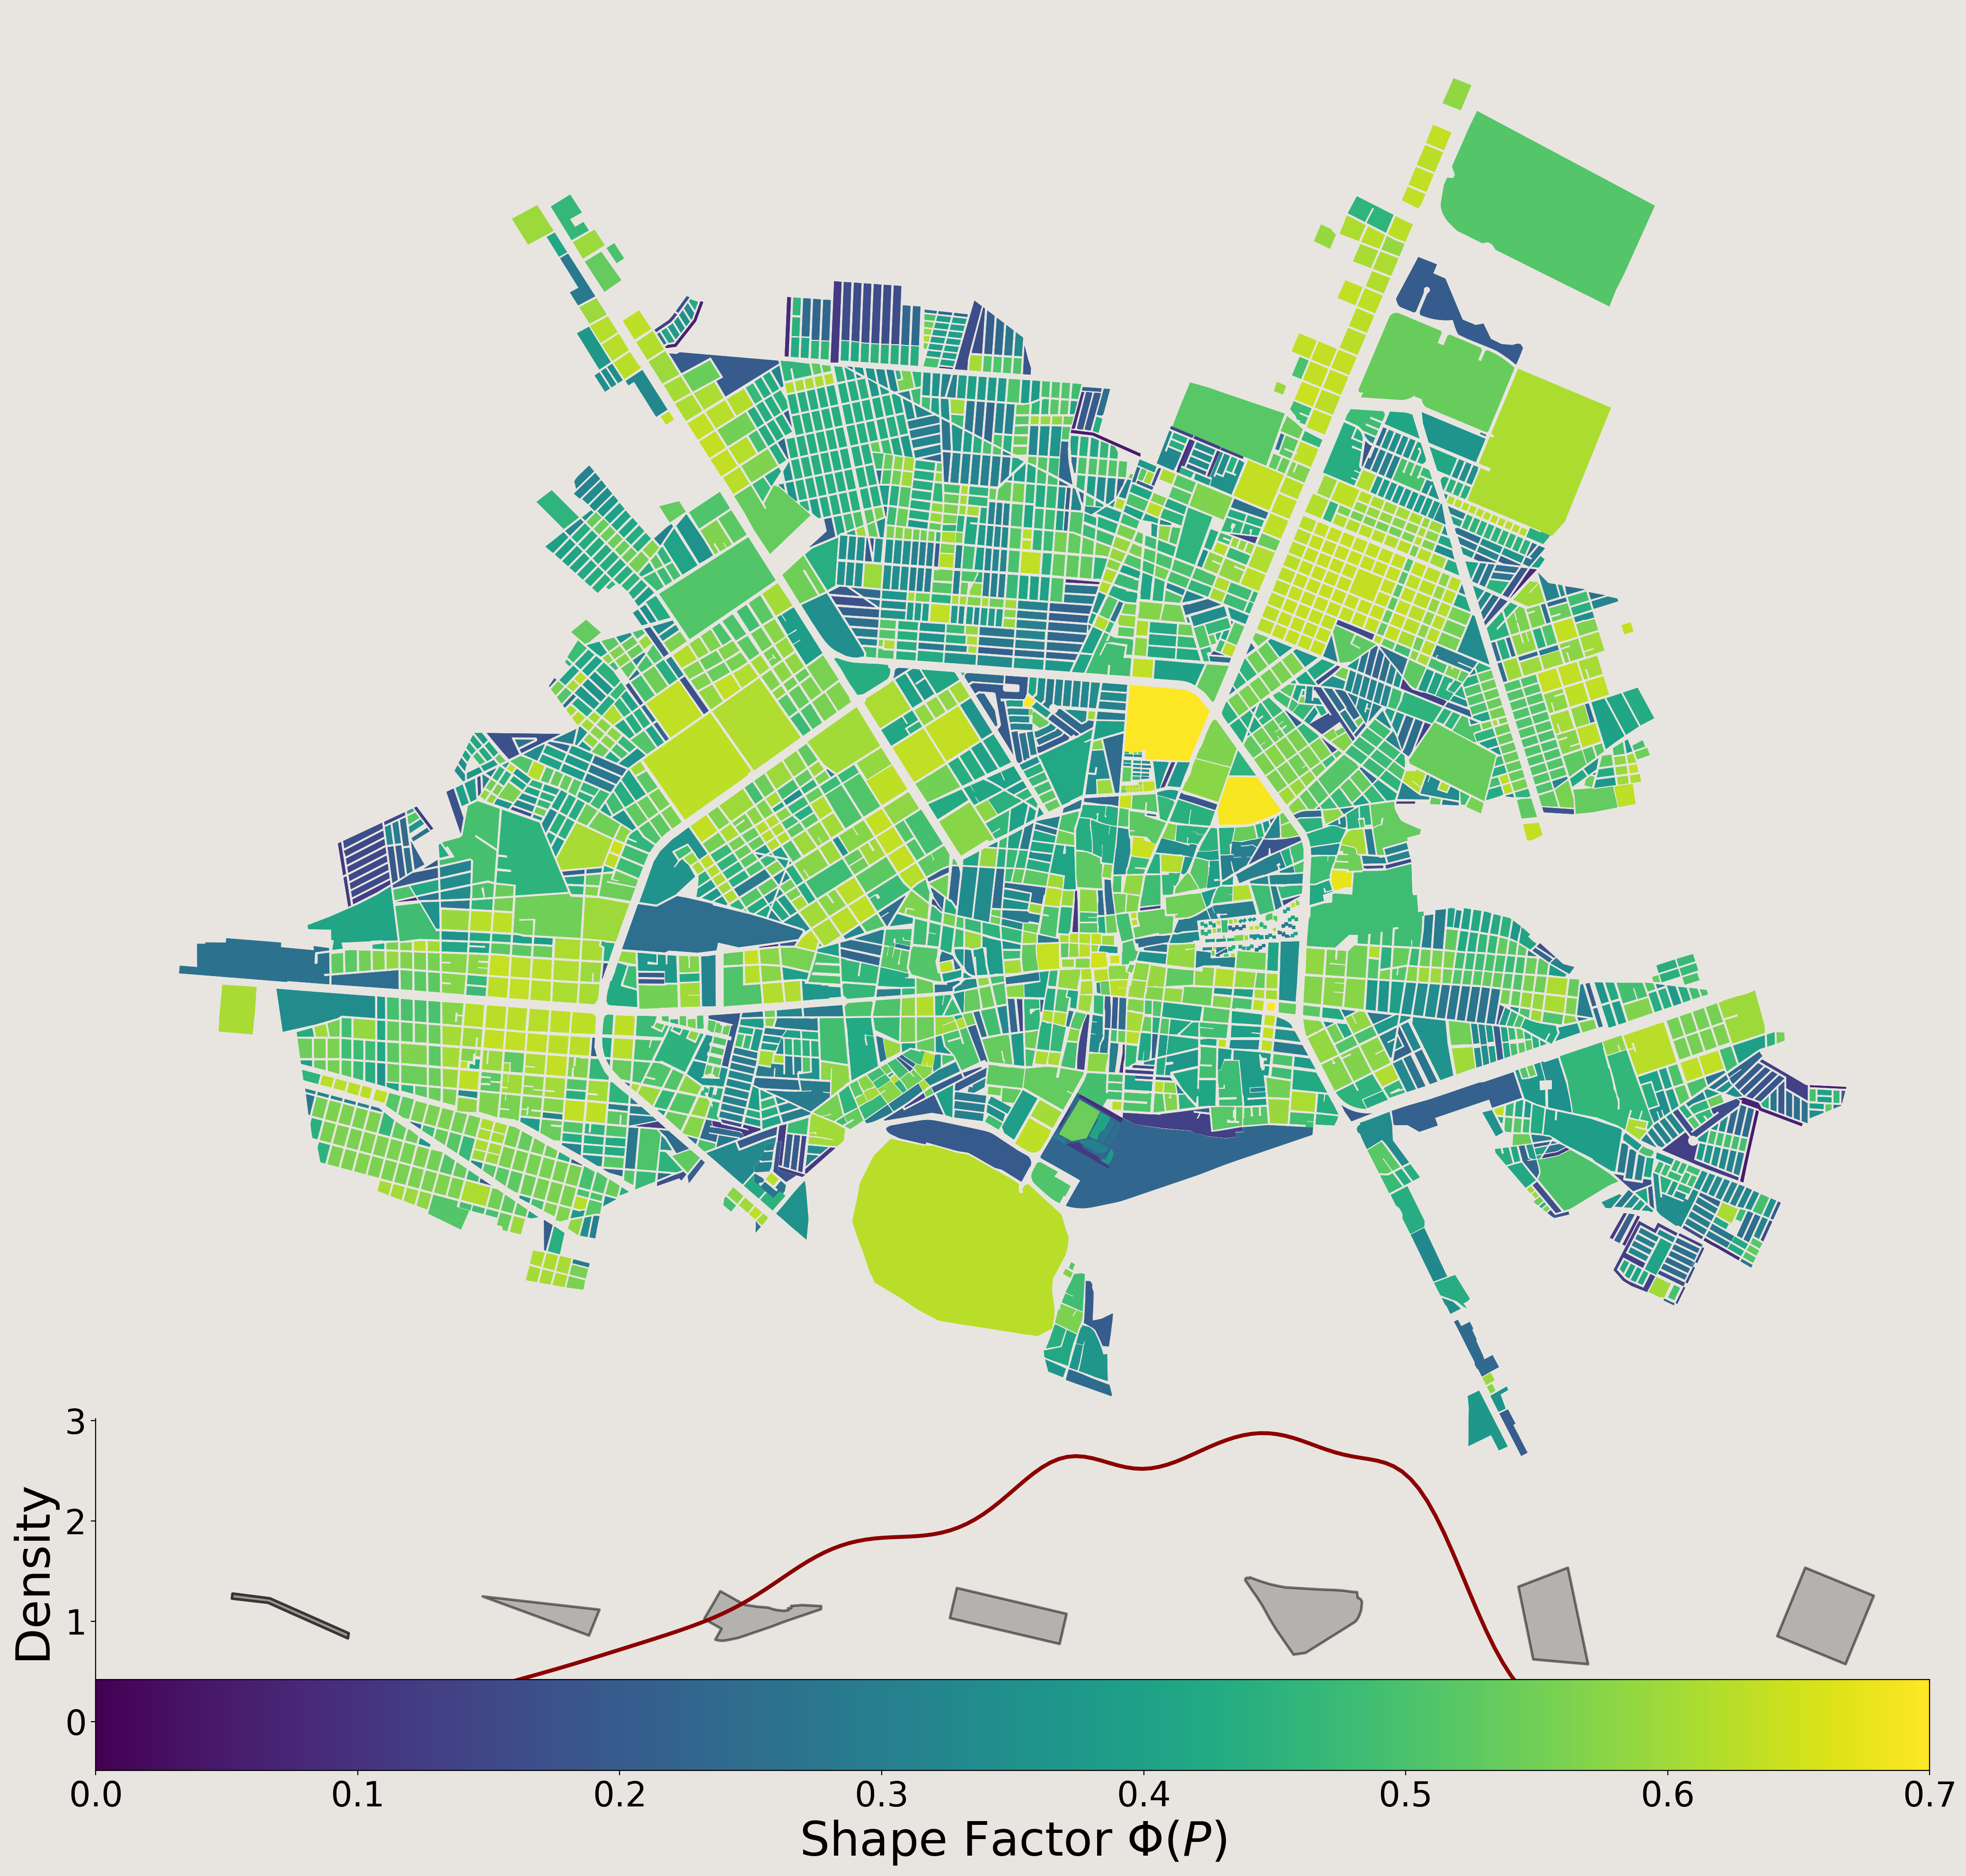
\includegraphics[width=0.88\linewidth]{Fig_ShapeFactor.png}
    \par{\centering \scriptsize Shape factor distribution of blocks in Fresnillo, Zac.\par}
\end{centering}

\vspace{0.4em}
\noindent\hspace{.2em} For two samples with empirical cumulative distribution functions (ECDFs) $F(x)$ and $G(x)$, the \textbf{Kolmogórov-Smirnov distance} $D_{KS}$ is
\[D_{KS} = \sup_{x} \left|F(x)-G(x)\right|\]
\begin{centering}
    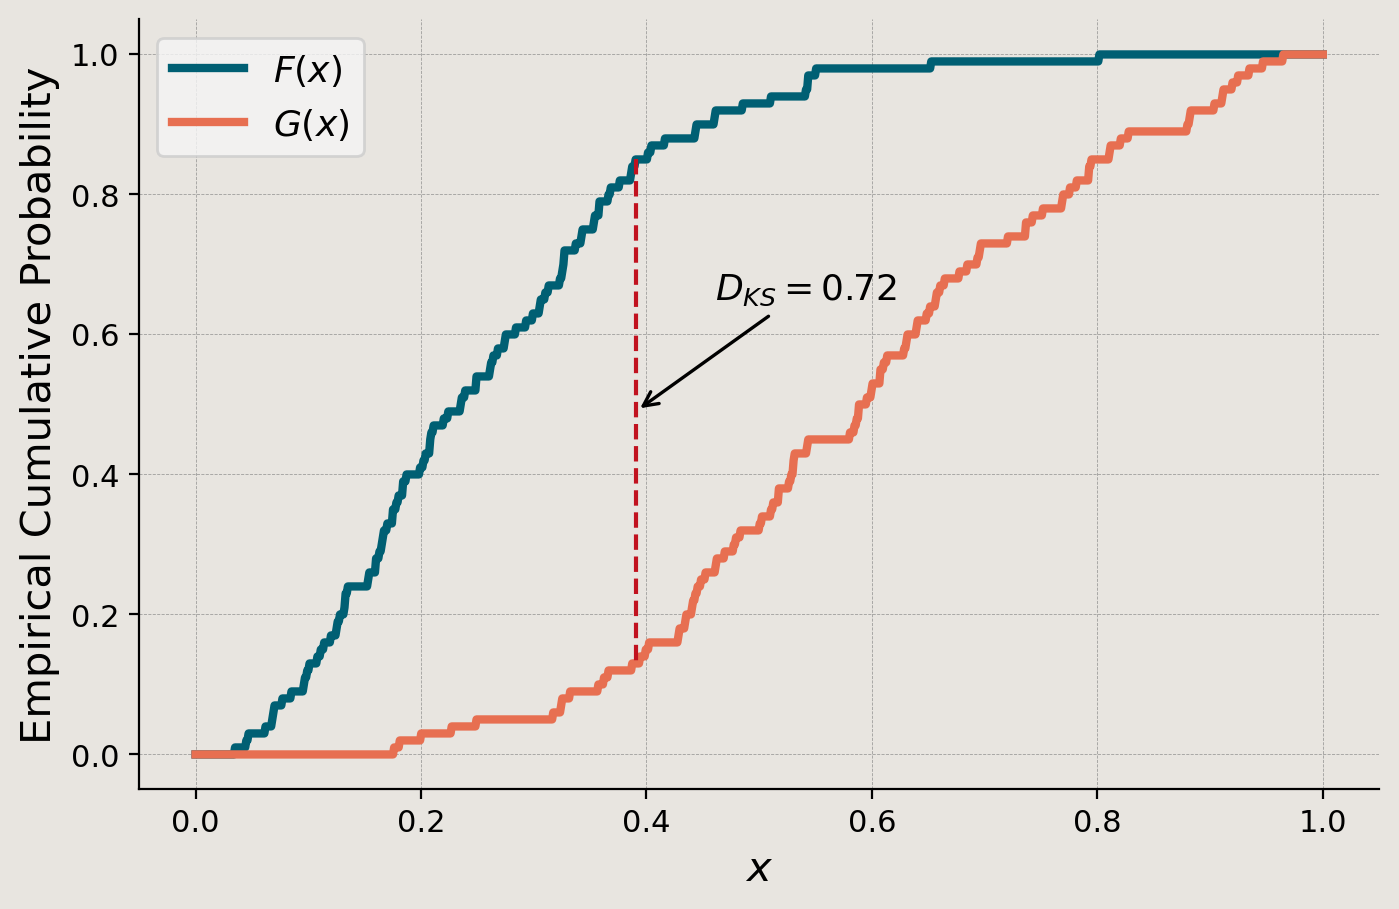
\includegraphics[width=0.85\linewidth]{KS.png}
   \par{\centering \scriptsize Kolmogórov–Smirnov Distance.\par}
\end{centering}
}

\headerbox{\LARGE{\textbf{Methodology}}}{name=methodology,column=0,below=introduccion,span=2}{
\vspace{0.1cm}
\begin{enumerate}
    \item Extract the \textbf{street network} of each of the 40,810 human settlements in Mexico using geospatial data from INEGI \cite{Maravillo2023}.
    \item Compute the \textbf{distribution of the block shape factor} $\Phi(P)$ for Mexican cities containing at least 100 blocks (2,591 urban areas in total).
    \item  Construct a pairwise \textbf{Kolmogórov–Smirnov distance matrix} to quantify dissimilarities between the shape factor distributions of all urban areas.
    
    \item Apply the \textbf{$k$-medoids clustering algorithm} to classify cities according to the geometric properties of their street networks.
    
    \item Estimate an appropriate number of clusters ($k^{*}$) using the \textbf{elbow method} based on \textbf{clustering inertia}.

    \item Use the \textbf{UMAP algorithm \cite{McInnes2018}} (\textit{Uniform Manifold Approximation and Projection}), a topological dimensionality-reduction technique, to visualize the resulting urban typology.
\end{enumerate}
}


\headerbox{\LARGE{\textbf{Results}}}{name=result,column=0,span=3,below=methodology}{
\noindent
\begin{minipage}[t]{0.54\linewidth}\vspace{0pt}
  \centering
  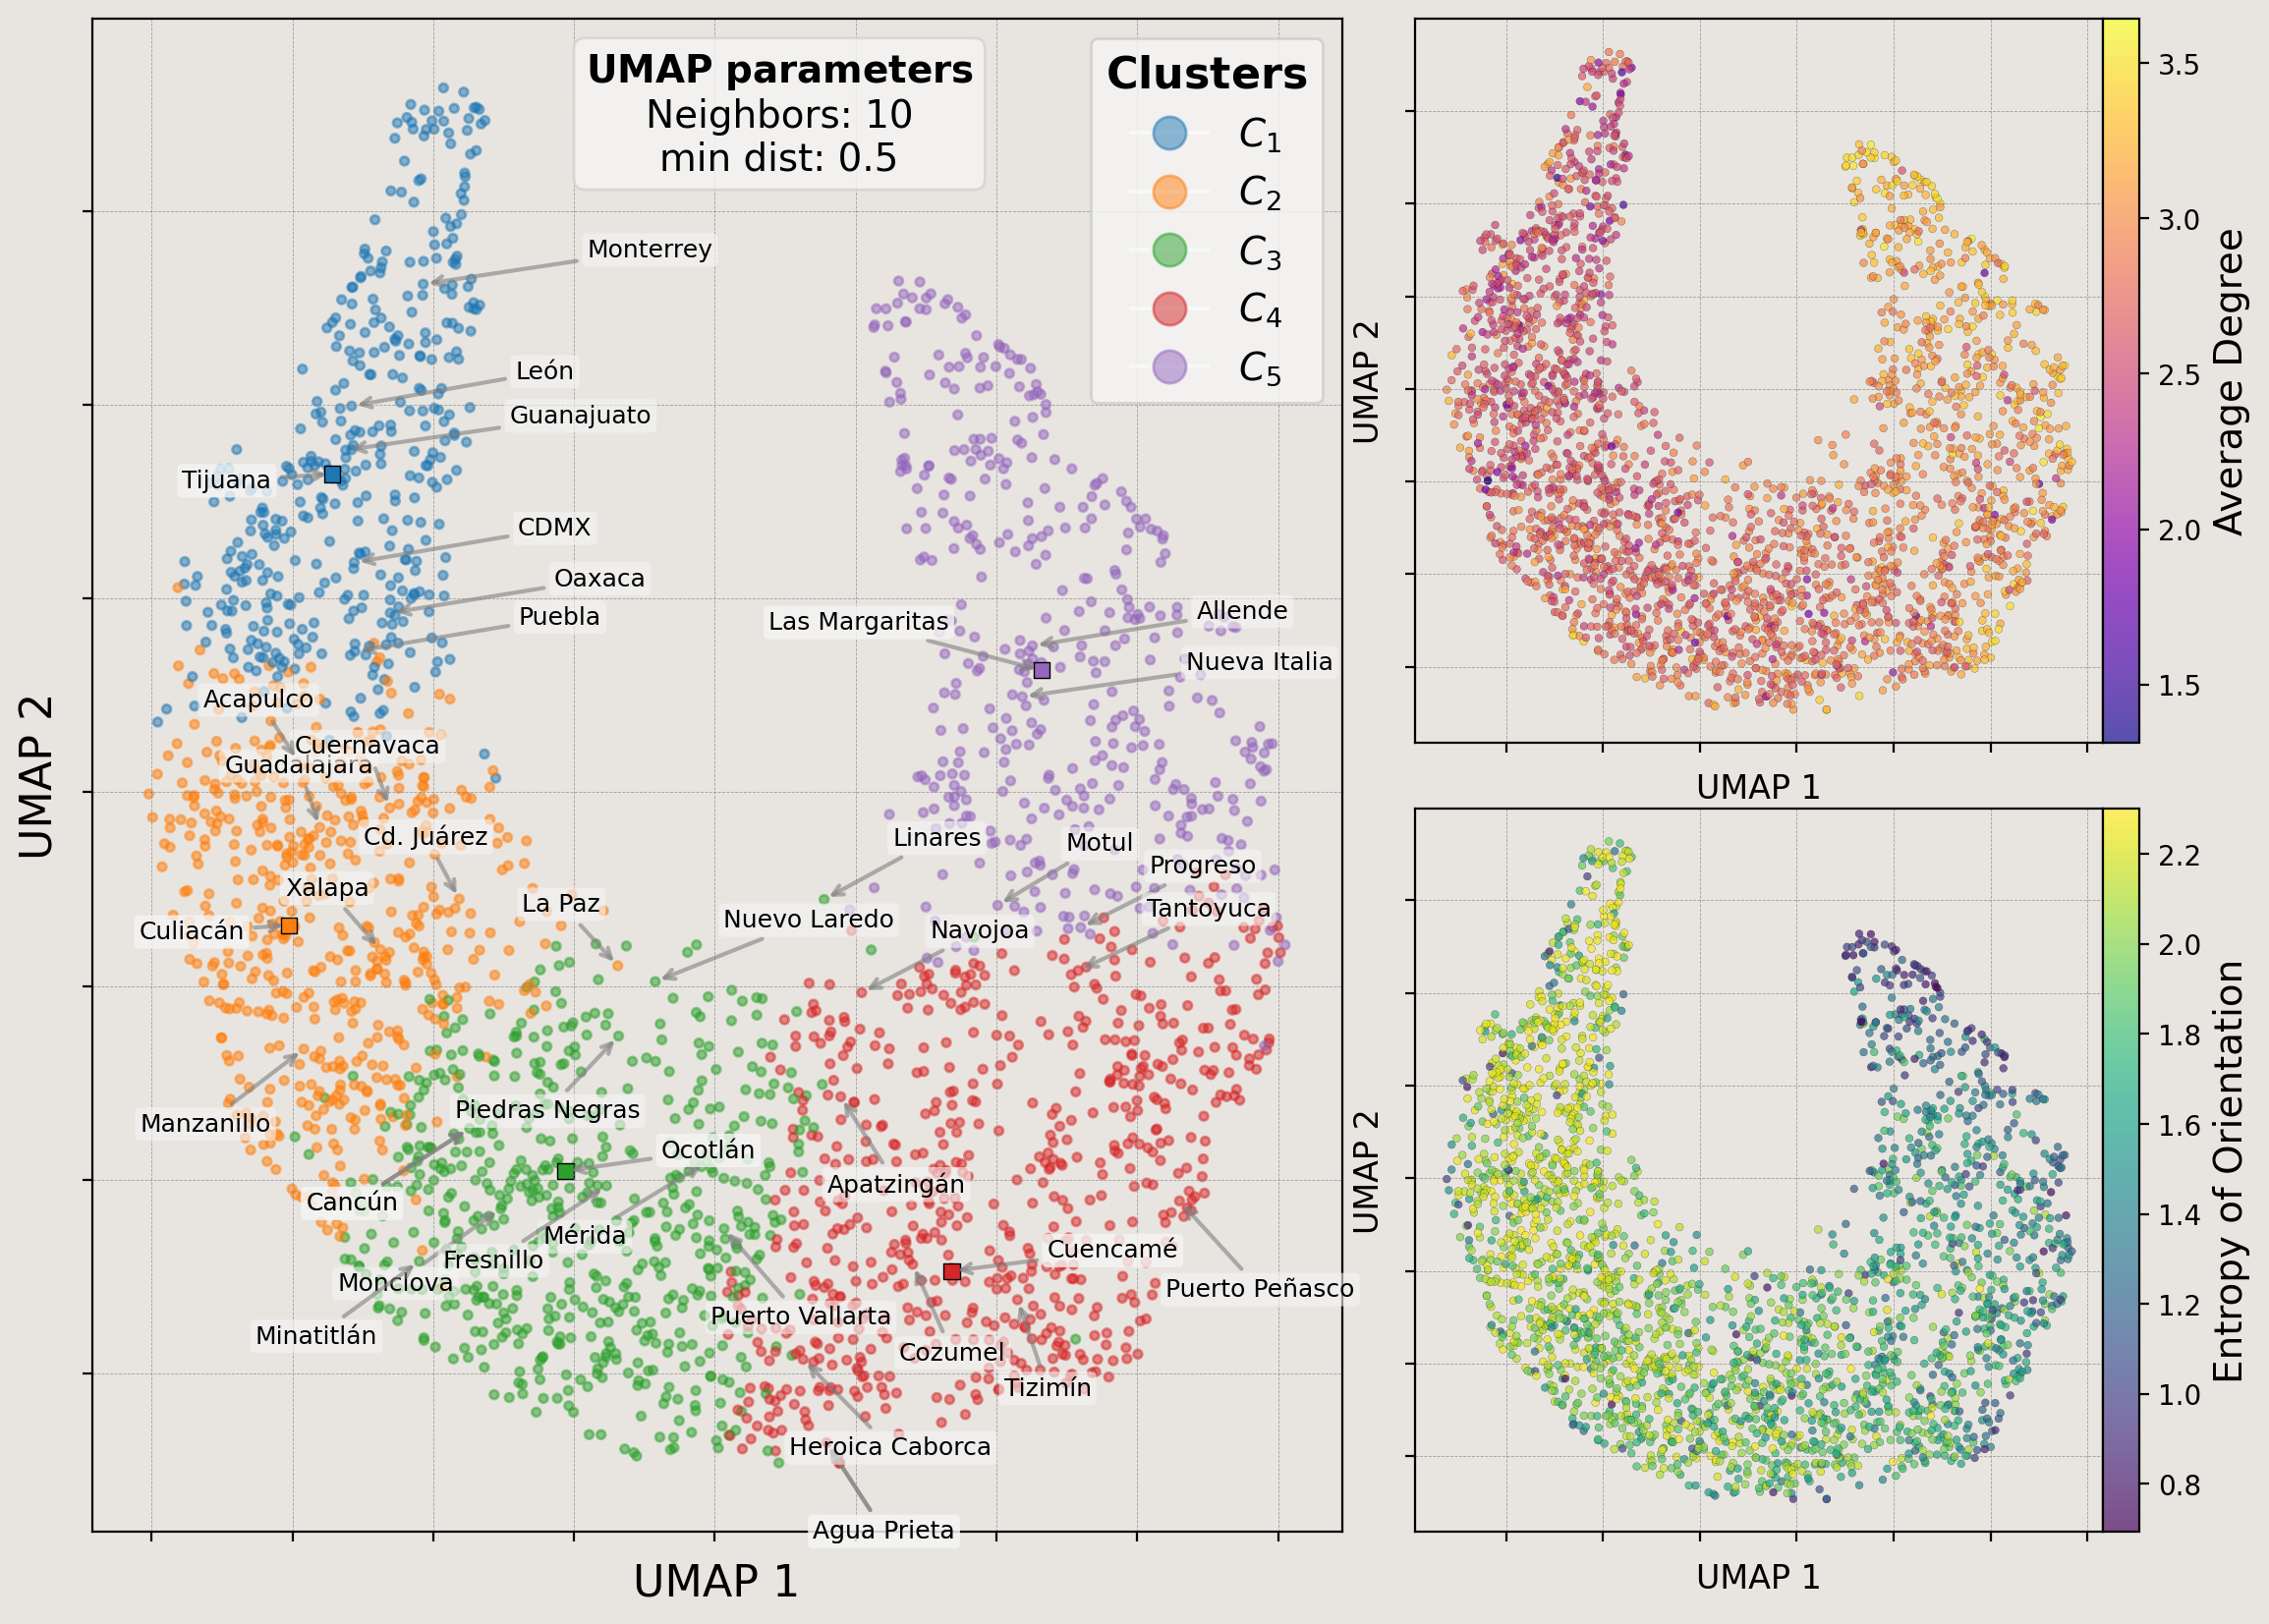
\includegraphics[width=\linewidth]{UMAP2.png}
  {
  \small{
  2D UMAP embedding of street networks based on shape factor distribution.}\\
  \vspace{1mm}

  \textit{Left:} $k$-Medoids classification. \textit{Top right:} Entropy distribution of street segment orientations. \textit{Bottom right:} Distribution of the average degree of street network.
  }
\end{minipage}
\hspace{0.0\linewidth}
\begin{minipage}[t]{0.45\linewidth}\vspace{0pt}
  \centering
  \begin{tabular}{cc}
    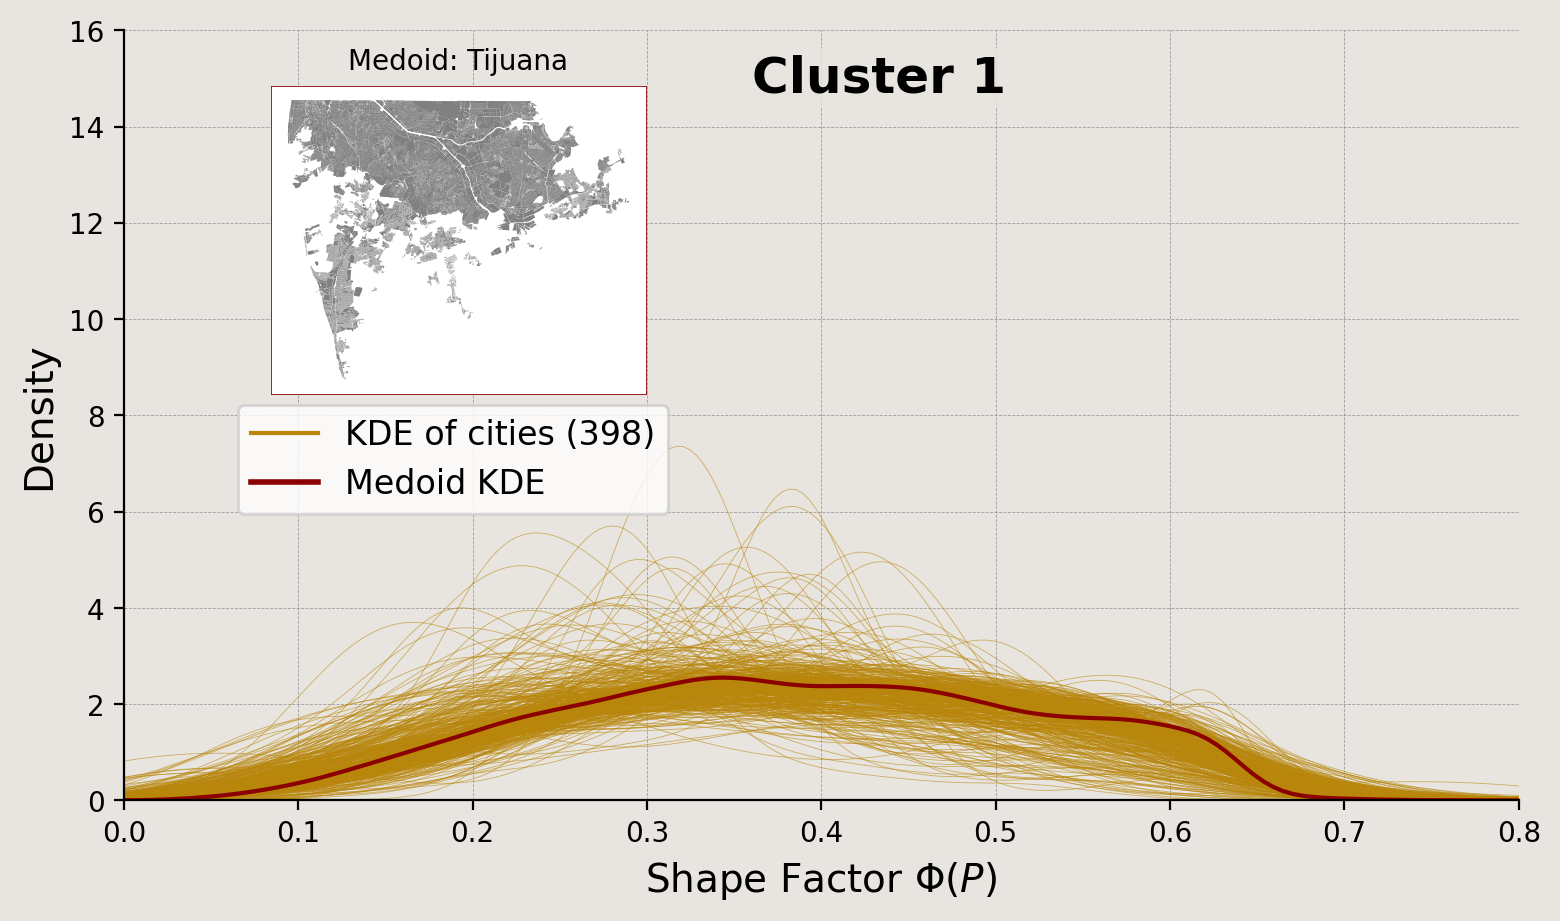
\includegraphics[width=0.44\linewidth]{Fig_Cluster_1.PNG} &
    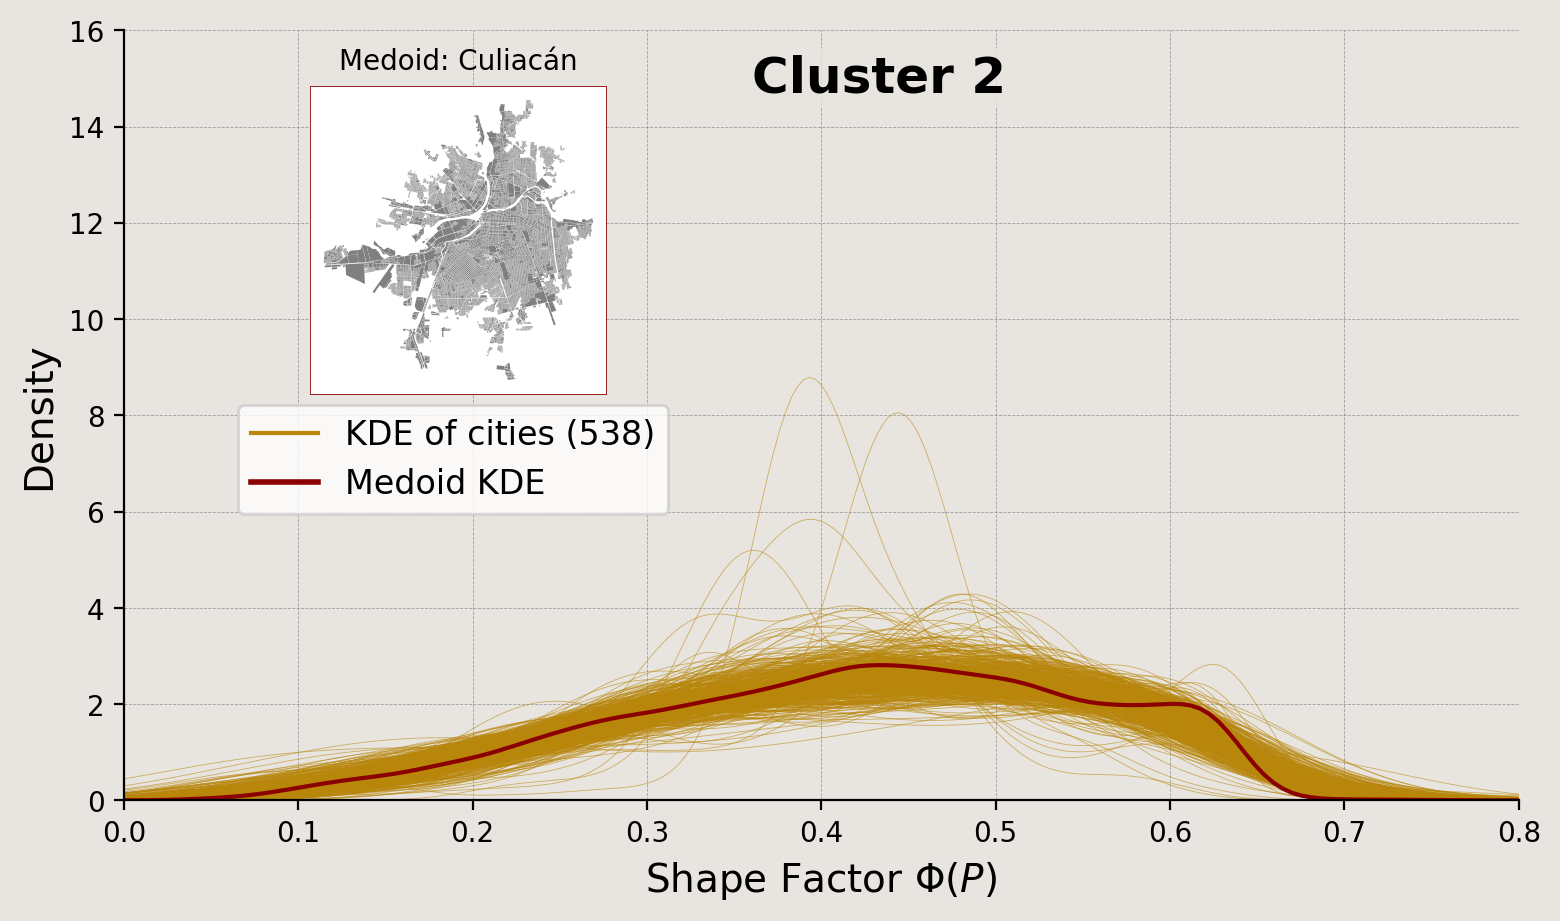
\includegraphics[width=0.44\linewidth]{Fig_Cluster_2.PNG} \\[0.9em]
    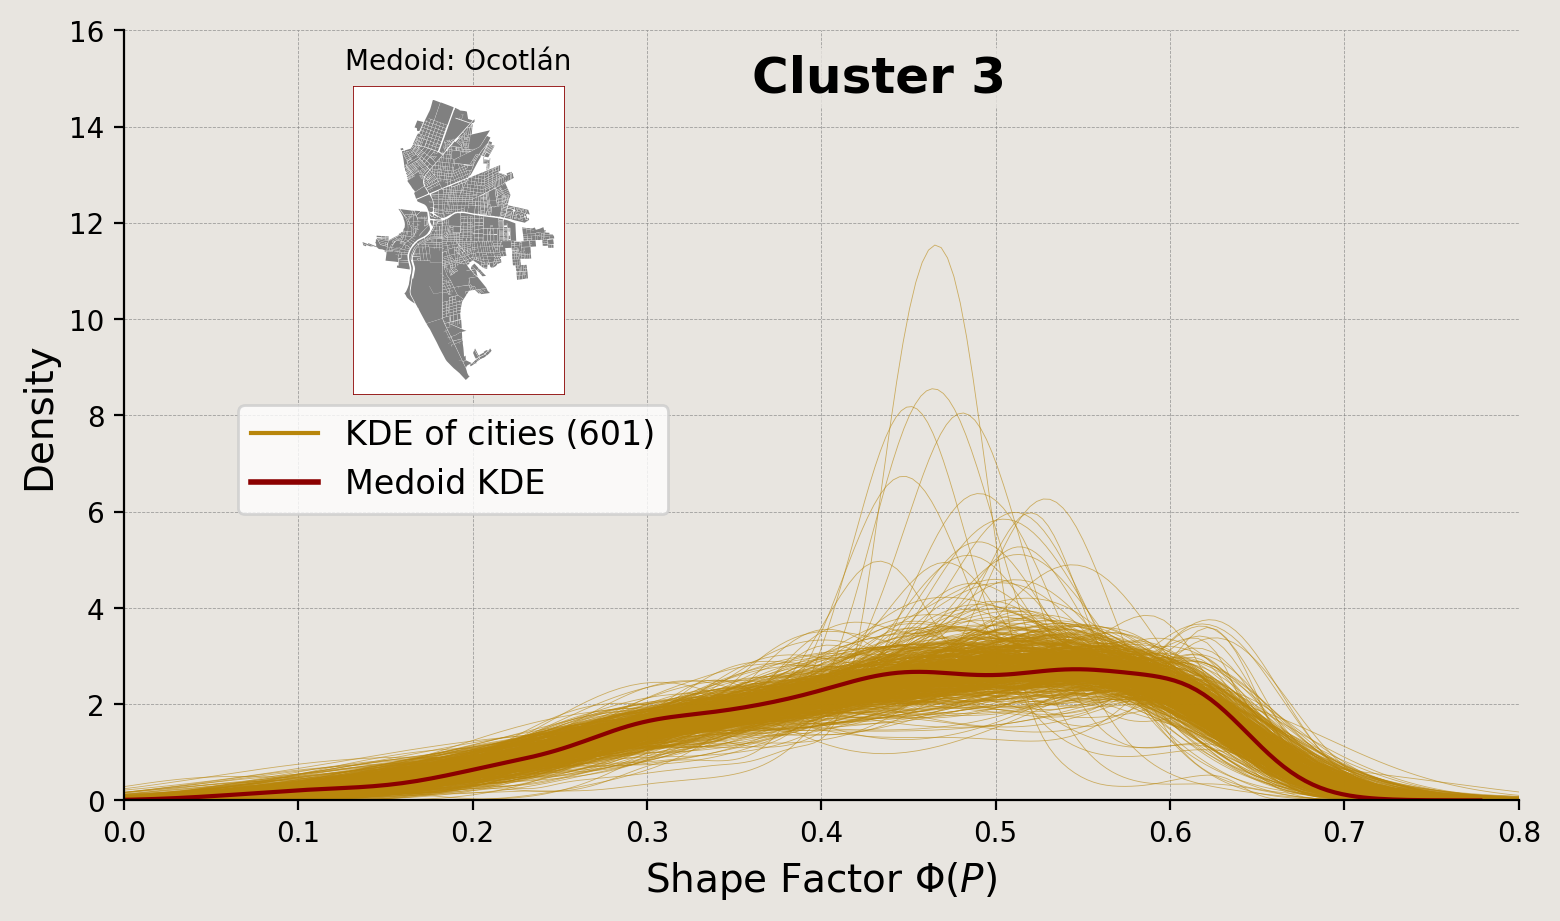
\includegraphics[width=0.44\linewidth]{Fig_Cluster_3.PNG} &
    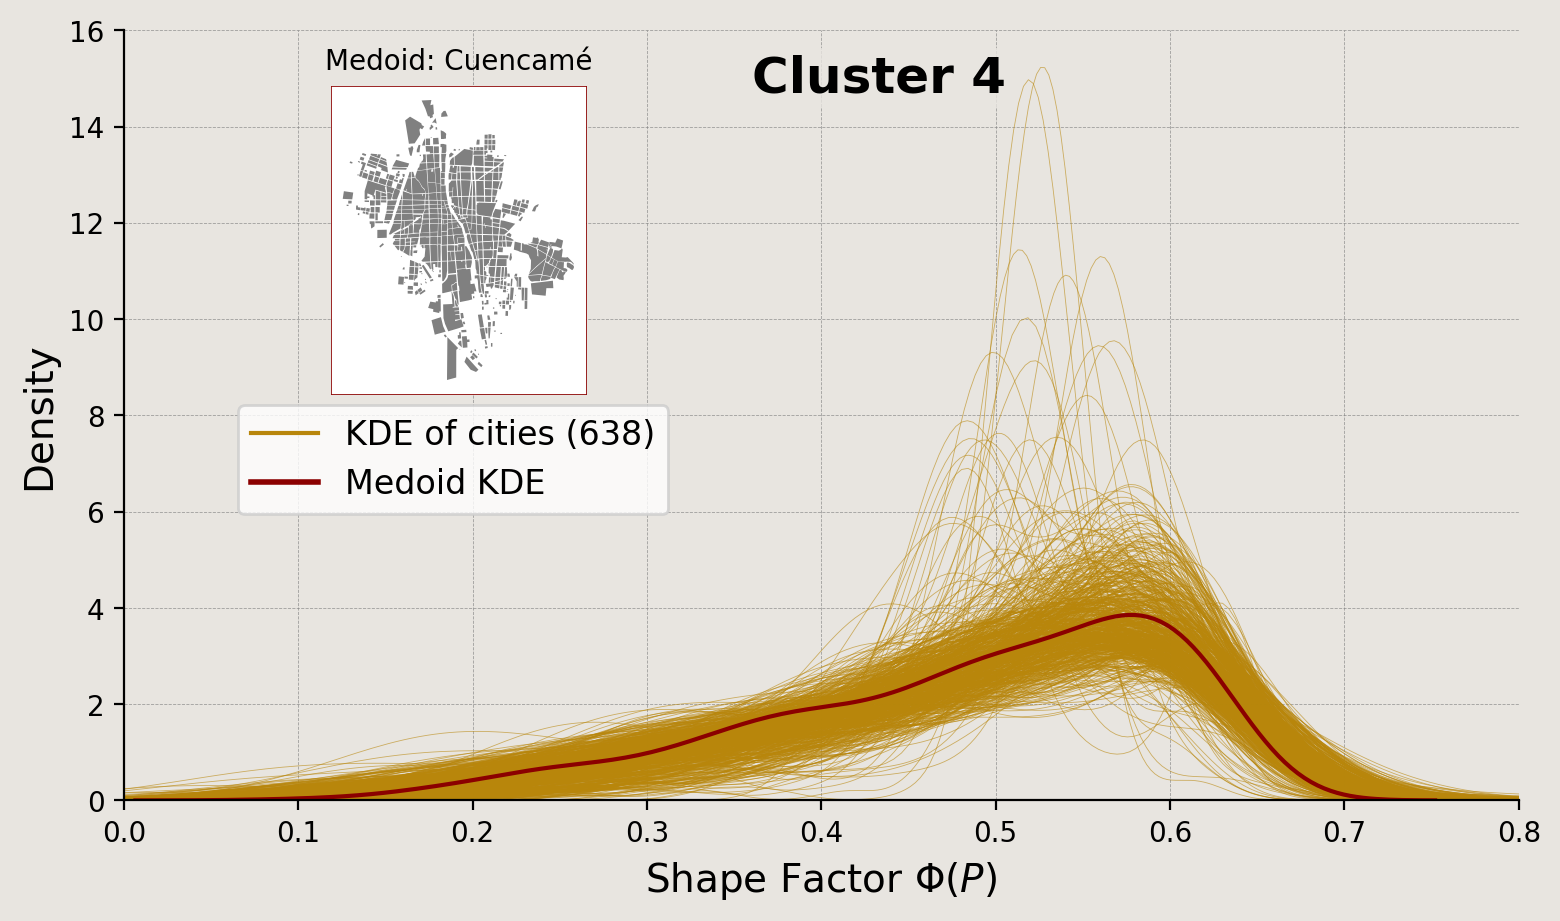
\includegraphics[width=0.44\linewidth]{Fig_Cluster_4.PNG} \\[0.9em]
     & 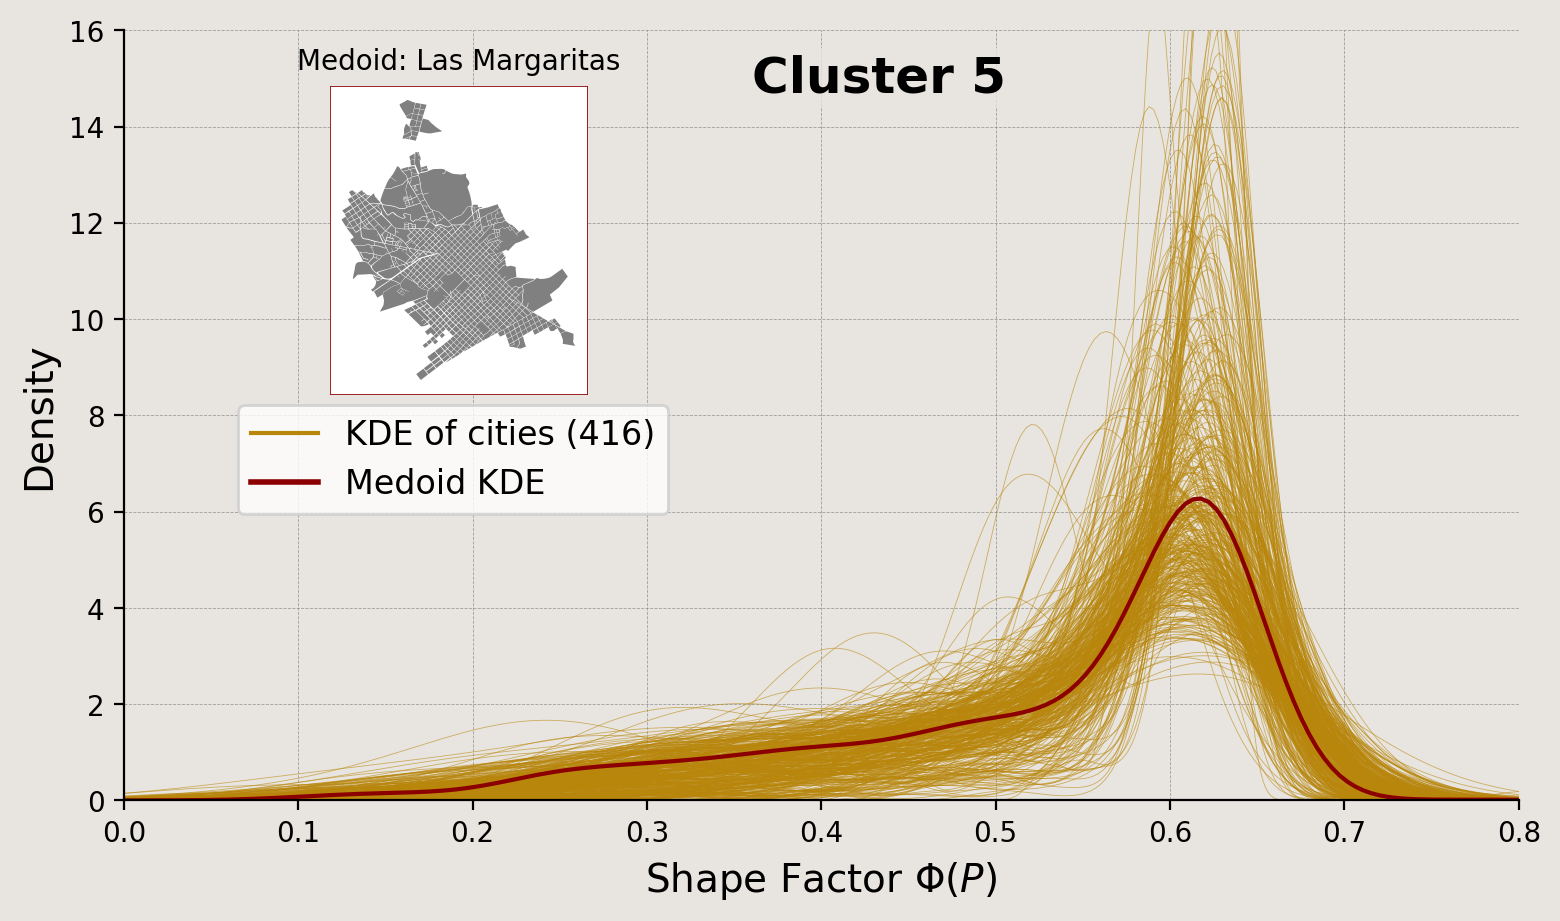
\includegraphics[width=0.44\linewidth]{Fig_Cluster_5.PNG} \\
  \end{tabular}
  {
    \small
    Morphological typologies of Mexican street layouts (KDE estimation of the distribution of block-shape distribution by cluster).
  }
\end{minipage}

}


\headerbox{\LARGE{\textbf{Conclusions}}}{name=conclusion,column=0,below=result,span=2,above=bottom}{

\vspace{0.1cm}
\begin{itemize}
    \item  The \textbf{full distribution of block shape factors} effectively captures the geometric and topological properties of the street layout.
    \item The \textbf{Kolmogórov–Smirnov distance} provides an alternative approach  to clustering data without relying on summary-statistic representations.
    \item \textbf{Five} main \textbf{morphological classes of Mexican cities} were identified, ranging from irregular street layouts characterized by blocks of diverse shapes  to highly ordered cities with grid-like street networks.
\end{itemize}
\vspace{.1cm}

}

\headerbox{\LARGE{\textbf{References}}}{name=references,column=2,below=result,span=1,above=bottom}{
\renewcommand{\refname}{} 
\vspace{-0.3cm} 
\scriptsize
\begin{thebibliography}{99}\compresslist
%\bibitem{Strano2013}
%E. Strano, M. Viana, L. da Fontoura, A. Cardillo, S. Porta, V. Latora. \textit{Urban street networks, a comparative analysis of ten European cities.}
%Environment and Planning B, 40(6), 2013.

\bibitem{McInnes2018}
L. McInnes, J. Healy \& J. Melville UMAP: Uniform manifold approximation and projection for dimension reduction. \textit{arXiv preprint}, 1802.03426, 2018.

\bibitem{Boeing2019}
G. Boeing.  Urban spatial order: Street network orientation, configuration, and entropy. \textit{Applied Network Science}, 4(1), 2019.

\bibitem{Badhrudeen2022}
M. Badhrudeen, S. Derrible, T. Verma, A. Kermanshah \& A. Furno. A geometric classification of world urban road networks. \textit{Urban Science}, 6(1), 2022.

%\bibitem{Strano2012}
%E. Strano, V. Nicosia, V. Latora, S. Porta, M. Barthélemy. \textit{Elementary processes governing the evolution of road networks.} Scientific Reports, 2(1), 2012.

\bibitem{Maravillo2023}
H. Maravillo, G. Calvillo \& E. Treviño. X The population size of Mexican cities follows a power-law distribution.
\textit{Mathematical Population Studies}, 30(4), 2023.
\end{thebibliography}
}\textit{}


\end{poster}

\end{document}
